\documentclass[
    10pt,
    aspectratio=169,
    xcolor={dvipsnames},
    spanish,
    % handout,
    % notes=only,
    % notes,
    ]{beamer}

% BEAMER SETTINGS
\setbeamerfont{section in toc}{size=\normalsize, shape=\bfseries}
\mode<presentation>{
    \usetheme{Antibes}
    \setbeamercovered{transparent}
    \usecolortheme{rose}
    \setbeamertemplate{navigation symbols}{}
    }

% PACKAGES
% \usepackage[spanish]{babel}  % uncomment for Spanish support
\usepackage{tikz,pgfplots}
\pgfplotsset{compat=1.13}
\usetikzlibrary{calc}
% arrows.meta provides modern arrow tips (and avoids unknown 'Latex' tip errors)
\usetikzlibrary{arrows.meta}
\usepackage{subcaption}
\usepackage{graphicx}
\graphicspath{{figures/}}
\usepackage{booktabs}
\usepackage{upgreek}
\usepackage{commath}
\usepackage{amsmath,amsthm,amssymb,mathtools,mathrsfs}
\usepackage{cancel}
\usepackage{fontawesome5}
\usepackage{enumerate}
\usepackage{tensor}
\usepackage[font=footnotesize]{caption}
\usepackage{wasysym}
\usepackage[skins,theorems]{tcolorbox}
\tcbset{
    highlight math style={
        enhanced,
        coltext=black,
        colframe=black,
        colback=lightgray,
        arc=0pt,
        boxrule=.5pt
        }
}

% REFERENCES AND OTHERS
\usepackage{aas_macros}
\usepackage{natbib}
\bibpunct{(}{)}{;}{a}{}{,}

\usepackage{siunitx}
\sisetup{
    range-phrase=\text{--},
    range-units=single,
    separate-uncertainty=true,
    print-unity-mantissa=false
    }
\DeclareSIUnit{\gauss}{G}
\DeclareSIUnit{\jansky}{Jy}
\renewcommand{\figurename}{Fig.}

\usepackage{hyperref}
\hypersetup{
    % bookmarks=true,
    unicode=true,
    pdftoolbar=true,
    pdfmenubar=true,
    pdffitwindow=false,
    pdfstartview={FitH},
    pdftitle={ISI-Free Linear Combination Pulses with Better Performanc},
    pdfauthor={Erik Saez A.},
    pdfcreator={Erik Saez A.},
    pdfnewwindow=true,
    colorlinks=true,
    linkcolor=RoyalBlue,
    citecolor=RoyalBlue,
    urlcolor=RoyalBlue
    }

\title[Auxiliar \#5 - MAS/Ondas]{\bfseries Auxiliar \#5 - MAS/Ondas}
\subtitle{Introducción a la Física Moderna (F1100-5)}
\author[Erik Saez A.]{Erik Saez A. - Javiera Toro}
\institute[UChile]{Departamento de Ingeniería Eléctrica \\ Universidad de Chile}

\date{\today}

\begin{document}

\begin{frame}
  \titlepage
  \centering
  \faIcon{envelope} \href{mailto:erik.saez@ug.uchile.cl}{erik.saez@ug.uchile.cl} \hspace{.2cm}
\end{frame}

\begin{frame}{Contenidos}
  \tableofcontents
\end{frame}

\section{Resumen MAS}

% ====== Frame 1: MAS (distribución 2x2, compacto y simétrico) ======
\begin{frame}{M.A.S.: Ecuación y Solución}
  \footnotesize
  \begin{columns}[T]
    \begin{column}{0.58\textwidth}
      \begin{block}{EDO del M.A.S.}
        Una \textbf{ecuación diferencial ordinaria (EDO)} relaciona una función   desconocida y sus derivadas respecto de una sola variable independiente. La forma más común que encontraremos es la EDO lineal homogénea de 2° orden:
        \begin{equation*}
          m\ddot x + kx = 0 \;\Longleftrightarrow\; \ddot x + \frac{k}{m}x = 0
        \end{equation*}
        \noindent Frecuencia angular $\omega^2=\tfrac{k}{m} \;\Rightarrow\; \omega=\sqrt{\tfrac{k}{m}}$, que cuantifica la rapidez de la oscilación.\vspace{-2pt}
      \end{block}
      \begin{block}{Posición de equilibrio}
        La \textbf{posición de equilibrio} $x_{\text{eq}}$ es aquella en la que la fuerza neta (y por ende la aceleración) se anula: $m\ddot x=0$, lo que implica que:\begin{align}
          \ddot{x}= \dot{x} = 0
        \end{align}
      \end{block}
    \end{column}
    \begin{column}{0.45\textwidth}
      \begin{block}{Derivadas útiles}
        Cambio de variable respecto al equilibrio:\\[-2pt]
        \[
          \begin{aligned}
            y(t) &= x(t)-x_{\text{eq}},\\
            \dot y(t) &= \dot x(t),\\
            \ddot y(t) &= \ddot x(t).
          \end{aligned}
        \]
      \end{block}
      \begin{block}{Solución general y derivada (conocida)}
        Para $\ddot x + \omega^2 x=0$:
        \[
          \begin{aligned}
            x(t) &= A\cos(\omega t)+B\sin(\omega t),\\
            \dot x(t) &= -A\omega\sin(\omega t)+B\omega\cos(\omega t).
          \end{aligned}
        \]
        C.I.: $x(t= 0)=x_0 \Rightarrow A=x_0$, $\;\dot x(0)=v_0 \Rightarrow B=v_0/\omega$.
      \end{block}
    \end{column}
  \end{columns}
\end{frame}
\section{Resumen Ondas}
% ====== Frame 2: Ondas: viajeras y superposición (2x2 equilibrado) ======
\begin{frame}{Ondas en cuerdas: viajeras y superposición}
  \footnotesize
  \begin{columns}[T,totalwidth=\textwidth]
    % ---------- Columna izquierda ----------
    \begin{column}{0.4\textwidth}
      \begin{block}{Ecuación de onda y velocidad}
        La ecuacion de la onda describe el comportamiento temporal y espacial de perturbaciones que se propagan en un medio.
   
        \[
          \frac{\partial^{2}y}{\partial t^{2}}
          = c^{2}\,\frac{\partial^{2}y}{\partial x^{2}},
          \qquad c=\sqrt{\tfrac{T}{\rho}}.
        \]
    
      \end{block}
      \begin{block}{Soluciones de d’Alembert}
        La solucion de la ecuación de onda es:
    
        \[
          y(x,t)=f(x-ct)+g(x+ct).
        \]
        \begin{itemize}
          \item \textbf{Derecha:} $f(x-ct)$ (traslación en $+x$).
          \item \textbf{Izquierda:} $g(x+ct)$ (traslación en $-x$).
        \end{itemize}
     
      \end{block}
    \end{column}
    % ---------- Columna derecha ----------
    \begin{column}{0.5\textwidth}
      \begin{block}{Onda armónica viajera}
       
        \begin{align}
          y(x,t)=A\cos(kx-\omega t+\phi)\\
          k=\tfrac{2\pi}{\lambda},\quad c=\tfrac{\omega}{k}=\tfrac{\lambda}{T}
        \end{align}
          
      \end{block}
      \begin{block}{Superposición / Interferencia (misma $k,\omega$)}
      
        \[
          y_1=A\cos\Theta,\quad
          y_2=A\cos(\Theta+\Delta\phi),\qquad
          \Theta=kx-\omega t+\phi.
        \]
        Suma:
        \[
          y=y_1+y_2=
          2A\cos\!\Big(\tfrac{\Delta\phi}{2}\Big)\,
          \cos\!\Big(\Theta+\tfrac{\Delta\phi}{2}\Big).
        \]
        Casos clave:
        \begin{itemize}
          \item \textbf{En fase} ($\Delta\phi=0$): amplitud $=2A$ (constructiva).
          \item \textbf{En contrafase} ($\Delta\phi=\pi$): amplitud $=0$ (destructiva).
        \end{itemize}
  
      \end{block}
    \end{column}
  \end{columns}
\end{frame}



% ===================================

% =====================================
\section{Pregunta 1}

% ------------------ Ejercicio 1 ------------------
\begin{frame}{Ejercicio 1}
\begin{block}{Enunciado}
  \footnotesize
  Un péndulo de longitud $L$ con una masa $M$ está unido lateralmente a un resorte de constante elástica $k$, como se muestra esquemáticamente. Cuando la masa cuelga verticalmente bajo el punto de suspensión, el resorte está sin deformación.
\begin{enumerate}
  \item Obtén una expresión aproximada para el período de oscilación del sistema para pequeñas amplitudes (linealiza las ecuaciones de movimiento).
  \item Supón $M=1{,}00\,\mathrm{kg}$ y que, en ausencia del resorte, el período del péndulo es $2{,}00\,\mathrm{s}$. Determina $k$ si el período del sistema acoplado es $1{,}00\,\mathrm{s}$.
\end{enumerate}

\begin{center}
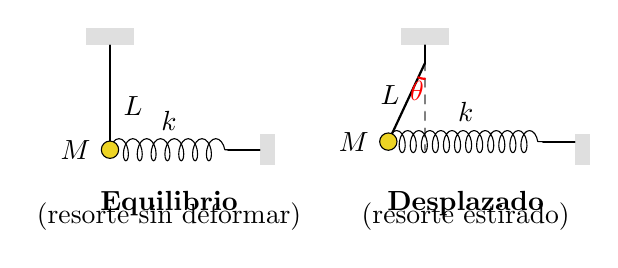
\begin{tikzpicture}[x=1cm,y=1cm,line cap=round,line join=round,>=latex,scale=0.5]
  % PRIMER DIAGRAMA - EQUILIBRIO
  \begin{scope}
    % Parameters
    \def\L{2.2}
    \def\spr{3.0}

    % Supports (simple blocks)
    \fill[gray!25] (-0.6,\L+0.45) rectangle (0.6,\L+0.9);
    \fill[gray!25] (\spr+0.8,-0.4) rectangle (\spr+1.2,0.4);

    % Hook and string (vertical)
    \draw[thick] (0,\L+0.45) -- (0,\L);
    \draw[thick] (0,\L) -- (0,0);

    % Spring sin deformar
    \draw[decorate,decoration={coil,segment length=5pt,amplitude=4pt}]
      (0,0) -- (\spr,0);
    % Small rod to wall
    \draw[thick] (\spr,0) -- (\spr+0.8,0);

    % Bob en equilibrio
    \fill[yellow!70!brown, draw=black] (0,0) circle (0.22);
    \node[left] at (-0.25,0) {$M$};

    % Labels
    \node[right] at (0.1,\L/2) {$L$};
    \node[above] at (\spr/2,0.25) {$k$};
    
    % Título
    \node[below] at (\spr/2,-0.8) {\textbf{Equilibrio}};
    \node[below] at (\spr/2,-1.1) {(resorte sin deformar)};
  \end{scope}

  % SEGUNDO DIAGRAMA - DESPLAZADO A LA IZQUIERDA
  \begin{scope}[xshift=8cm]
    % Parameters
    \def\L{2.2}
    \def\spr{3.0}  % Longitud natural del resorte
    \def\angle{-25}  % Ángulo negativo para desplazamiento a la izquierda
    \def\stretch{1.5}  % Factor de estiramiento del resorte (aumentado)

    % Supports (simple blocks)
    \fill[gray!25] (-0.6,\L+0.45) rectangle (0.6,\L+0.9);
    \fill[gray!25] (\spr+0.8,-0.4) rectangle (\spr+1.2,0.4);

    % Posición de equilibrio (línea punteada)
    \draw[thick,dashed,gray] (0,\L+0.45) -- (0,0);
    
    % Posición desplazada de la masa (hacia la izquierda)
    \coordinate (mass) at ({\L*sin(\angle)}, {\L-\L*cos(\angle)});
    
    % Hook and string (desplazada)
    \draw[thick] (0,\L+0.45) -- (0,\L);
    \draw[thick] (0,\L) -- (mass);

    % Spring estirado desde la masa hasta la pared (en la posición original)
    \draw[decorate,decoration={coil,segment length=4pt,amplitude=4pt}]
      (mass) -- (\spr,{\L-\L*cos(\angle)});
    % Small rod to wall (en la posición original)
    \draw[thick] (\spr,{\L-\L*cos(\angle)}) -- (\spr+0.8,{\L-\L*cos(\angle)});

    % Bob desplazado
    \fill[yellow!70!brown, draw=black] (mass) circle (0.22);
    \node[left] at ($(mass)+(-0.25,0)$) {$M$};

    % Ángulo theta (ahora hacia la izquierda)
    \draw[thick,red] (0,{\L-0.4}) arc[start angle=-90, end angle={\angle-90}, radius=0.4];
    \node[red] at (-0.2,{\L-0.7}) {$\theta$};

    % Labels
    \node[left] at (-0.4,{\L/2+0.3}) {$L$};
    \node[above] at ({(\L*sin(\angle)+\spr)/2},{\L-\L*cos(\angle)+0.25}) {$k$};
    
    % Título
    \node[below] at ({(\L*sin(\angle)+\spr)/2},-0.8) {\textbf{Desplazado}};
    \node[below] at ({(\L*sin(\angle)+\spr)/2},-1.1) {(resorte estirado)};
  \end{scope}
\end{tikzpicture}
\end{center}
\end{block}
\end{frame}
\section{Pregunta 2}

%-------------------------------------
\begin{frame}{Ejercicio 2}
  \begin{block}{Enunciado}
    \begin{enumerate}
  \item Bosquee la función
  \begin{equation}
    f(x) = \frac{1\,\mathrm{cm}}{1 + \left(x/1\,\mathrm{cm}\right)^2}.
  \end{equation}
  Escriba $f(\bar{x})$ para $\bar{x} = x - ct$, donde $c$ es la velocidad de propagación de la onda y $t$ el tiempo. Si $c = 1\,\mathrm{cm/s}$, bosquee la función $u(x,t) = f(x-ct)$ para $t = 0, 1, 2\,\mathrm{s}$, donde $u(x,t)$ representa la amplitud de la onda en la posición $x$ y tiempo $t$.

  \item Calcule la velocidad vertical $v(x,t)$ de la cuerda en el instante $t = 0$. Para esto, derive la función $u(x,t)$ con respecto al tiempo considerando $x$ constante.

  \item Grafique $v(x,0)$ en función de $x$. Note que esta es positiva y negativa en ciertas partes. Interprete el resultado.
\end{enumerate}
    
  \end{block}
\end{frame}
% ------------------ Ejercicio 2 ------------------
\section{Pregunta 3}
% ------------------ Ejercicio 3 ------------------
\begin{frame}{Ejercicio 3}
  \footnotesize
  \begin{block}{Enunciado}
    Se tiene una masa $m$ sostenida de dos cuerdas de largos $L_1$ y $L_2$, con tensiones $T_1$ y $T_2$ respectivamente en presencia de gravedad, como se observa en la figura. Considere que $T_2$ es conocido y $T_1$ es tal que el sistema no se mueve verticalmente.

Si inicialmente la masa se suelta desde el reposo a una distancia $x$,
\begin{enumerate}
  \item Calcule el valor de $T_1$ para que el sistema no se mueva verticalmente.
  \item Encuentre la frecuencia angular de oscilación.
  \item Calcule el período de oscilación.
  \item Calcule la amplitud de oscilación de la masa.
\end{enumerate}
Considere para sus cálculos y aproximaciones $x \ll L_1, L_2$, y que las tensiones se mantienen al deformarse la cuerda.
\begin{figure}
\centering
% Reduce the tikzpicture scale so the whole figure fits the slide and avoid clipping
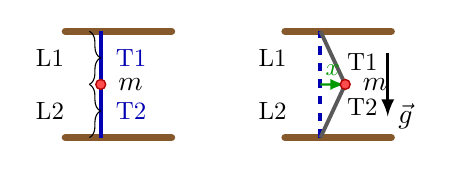
\begin{tikzpicture}[scale=0.45,%
  >=latex,
    board/.style={line width=2.6pt, draw=brown!70!black, line cap=round},
    stringV/.style={line width=1.4pt, draw=blue!70!black},
    string/.style={line width=1.4pt, draw=gray!70!black},
    mass/.style={draw=red!70!black, fill=red!70, line width=0.5pt},
    note/.style={scale=0.9}
]

% ------------------- Panel izquierdo: cuerda vertical -------------------
\def\H{3}    % altura entre barras
\def\W{3}    % ancho de barras
\def\xs{1}   % x de la cuerda
\def\ym{1.5} % y de la masa
\def\r{0.14} % radio de la masa

% Barras
\draw[board] (0,\H) -- (\W,\H);
\draw[board] (0,0)  -- (\W,0);

% Cuerda vertical
\draw[stringV] (\xs,0) -- (\xs,\H);

% Masa (por encima de la cuerda)
\fill[mass] (\xs,\ym) circle (\r);
\node[anchor=west] at (\xs+\r+0.08,\ym) {$m$};

% Tensiones T1 y T2
\node[note,blue!70!black,anchor=west] at (\xs+0.18, {(\H+\ym)/2}) {T1};
\node[note,blue!70!black,anchor=west] at (\xs+0.18, {\ym/2})      {T2};

% Brazos L1 y L2 con llaves
\draw[decorate,decoration={brace,mirror,amplitude=4pt}]
  ([xshift=-0.32cm]\xs,\ym) -- ([xshift=-0.32cm]\xs,\H)
  node[midway,left=6pt,note] {L1};
\draw[decorate,decoration={brace,mirror,amplitude=4pt}]
  ([xshift=-0.32cm]\xs,0) -- ([xshift=-0.32cm]\xs,\ym)
  node[midway,left=6pt,note] {L2};

% ------------------- Panel derecho: masa desplazada -------------------
\begin{scope}[xshift=6.2cm]
  % Barras
  \draw[board] (0,\H) -- (\W,\H);
  \draw[board] (0,0)  -- (\W,0);

  % Línea de referencia vertical
  \draw[stringV,dashed] (\xs,0) -- (\xs,\H);

  % Coordenadas clave
  \coordinate (Top) at (\xs,\H);
  \coordinate (Bot) at (\xs,0);
  \coordinate (M)   at (\xs+0.70,\ym); % masa desplazada

  % Cuerdas inclinadas (detrás de la masa)
  \draw[string] (Top) -- (M);
  \draw[string] (Bot) -- (M);

  % Etiquetas T1 y T2
  \node[note,anchor=west] at ($(Top)!0.58!(M)+(0.10,0.00)$) {T1};
  \node[note,anchor=west] at ($(Bot)!0.58!(M)+(0.10,0.00)$) {T2};

  % Flecha x (debajo de la masa y acortada al borde)
  \draw[->,thick,green!60!black,shorten >=\r+0.02]
    (\xs,\ym) -- (M) node[midway,above,note] {$x$};

  % Doble referencia L1/L2 (solo texto)
  \node[note] at (-0.35, {(\H+\ym)/2}) {L1};
  \node[note] at (-0.35, {\ym/2})      {L2};

  % Masa dibujada al final (encima de cuerdas y flecha)
  \fill[mass] (M) circle (\r);
  \node[anchor=west] at ($(M)+(\r+0.08,0)$) {$m$};

  % ------------------- Flecha de gravedad (posicionada relativa a la masa)
  % Draw gravity arrow near the mass so it is inside the visible tikz area
  \draw[->,line width=1.1pt] ($(M)+(1.2,0.9)$) -- ($(M)+(1.2,-0.9)$) node[anchor=west] {$\vec g$};
\end{scope}
%

\end{tikzpicture}
\caption{Masa sostenida por dos cuerdas con tensiones $T_1$ y $T_2$.}
\end{figure}
\end{block}
\end{frame}
%--------------------------------------------
\section{Pregunta 4}
\begin{frame}{Ejercicio 4}
  \begin{block}{Enunciado}
En la siguiente figura se muestran dos pulsos, el pulso triangular se mueve hacia la derecha con una rapidez de $1~\mathrm{m/s}$ y el pulso rectangular se mueve hacia la izquierda también con una rapidez de $1~\mathrm{m/s}$. En el tiempo $t=0$, ambos pulsos están separados una distancia de $2~\mathrm{m}$.

\begin{enumerate}
  \item Considerando el sistema de referencia mostrado en la figura, escriba las funciones
  que representan al pulso triangular y al pulso rectangular por separado, para todo instante de tiempo.
  \item Dibuje el pulso resultante en los instantes $t=1,2,3,4~\mathrm{s}$. Considere que cuando
  dos ondas se encuentran, ambas ondas se suman.
\end{enumerate}

\begin{figure}[h!]
\centering
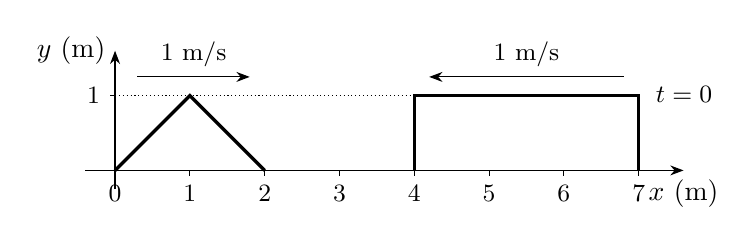
\begin{tikzpicture}[>=Stealth, scale=0.95]
  %----- Ejes
  \draw[->] (-0.4,0) -- (7.6,0) node[below] {$x$ (m)};
  \draw[->] (0,-0.25) -- (0,1.6) node[left] {$y$ (m)};

  %----- Marcas y valores en x
  \foreach \x in {0,1,2,3,4,5,6,7}{
    \draw (\x,0) -- (\x,-0.07) node[below] {\small \x};
  }
  % Marca en y=1 (y línea de referencia punteada)
  \draw (0,1) -- (-0.07,1) node[left] {\small 1};
  \draw[densely dotted] (0,1) -- (7,1);

  %----- Pulsos en t=0
  % Triangular (base 0..2, altura 1)
  \draw[line width=1.2pt] (0,0) -- (1,1) -- (2,0);
  % Rectangular (de 4 a 7, altura 1)
  \draw[line width=1.2pt] (4,0) -- (4,1) -- (7,1) -- (7,0);

  %----- Flechas de velocidad (1 m/s)
  \draw[->] (0.3,1.25) -- (1.8,1.25) node[midway, above] {\small $1~\mathrm{m/s}$};
  \draw[<-] (4.2,1.25) -- (6.8,1.25) node[midway, above] {\small $1~\mathrm{m/s}$};

  %----- Etiqueta t=0
  \node[right] at (7.1,1.02) {\small $t=0$};
\end{tikzpicture}
\caption{Condición inicial con marcas y valores en el eje $x$.}
\end{figure}
\end{block}
\end{frame}
%----------------------------
\section{Pregunta 5}
\begin{frame}{Ejercicio 5}
\begin{block}{Enunciado}
  Tres segmentos de cuerda de densidad $\mu$ están atados como muestra la figura. 
Suponga que se conocen las distancias $L_1$ y $L_2$, y el ángulo $\alpha$. 
Un pulso que parte en $A$ tarda un tiempo $T_B$ en llegar a $B$, y un tiempo $T_C$ en llegar a $C$. Encuentre la longitud de la cuerda $L_3$, y la tensión de la cuerda $L_1$.
\end{block}
\begin{figure}[h]
    \centering
    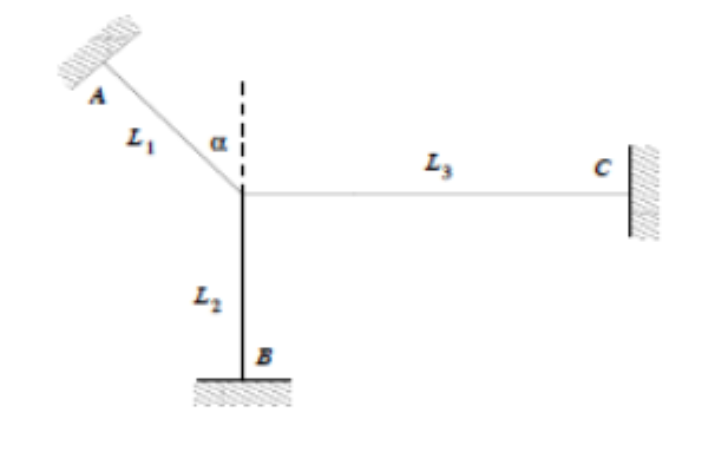
\includegraphics[width=0.4\textwidth]{Auxiliar_5_4}
    \caption{Esquema del sistema de cuerdas con segmentos $L_1$, $L_2$ y $L_3$ y ángulo $\alpha$.}
    \label{fig:cuerdas}
\end{figure}
\end{frame}
\begin{frame}{}
  \centering
  \Huge Éxito, ustedes son capaces de todo!
\end{frame}




\end{document}
